\documentclass[a4paper,12pt]{article}
\usepackage[hidelinks]{hyperref}
\usepackage{float}
\usepackage{graphicx}
\usepackage{listings}
\usepackage[utf8]{inputenc}
\usepackage{etoolbox}
\usepackage{fullpage}
\renewcommand*\contentsname{Indice}
\renewcommand*\figurename{Fig.}
\usepackage{setspace}
\usepackage{parskip}
\usepackage{subfigure}
\usepackage{amsmath}


\makeatletter
\patchcmd\l@section{%
  \nobreak\hfil\nobreak
}{%
  \nobreak
  \leaders\hbox{%
    $\m@th \mkern \@dotsep mu\hbox{.}\mkern \@dotsep mu$%
  }%
  \hfill
  \nobreak
}{}{\errmessage{\noexpand\l@section could not be patched}}
\makeatother

\setcounter{secnumdepth}{0}

% un po' di estetica...
\usepackage{fancyhdr}
\pagestyle{fancy}
\setlength{\headsep}{0.35in}
\let\MakeUppercase\relax

% blocchi di codice
\usepackage{listings}
\lstset{
	breaklines=true, 
	frame=single, 
	numbers=left,
	tabsize=2,
	basicstyle=\scriptsize,
	showstringspaces=false
}

\setlength{\parindent}{2em}
\setlength{\parskip}{0.5em}
\renewcommand{\baselinestretch}{1.5}

\fancyhf{} % clear all fields
\fancyfoot[C]{\thepage}

\frenchspacing

\begin{document}

\begin{titlepage}
\noindent
    \vspace*{5mm}
	\begin{minipage}[t]{0.15\textwidth}
	    \vspace*{5mm}
		\vspace{-3.5mm}{
\includegraphics[scale=1.8]{img/logo_bicocca.png}}
	\end{minipage}
	\hspace{1cm}
	\begin{minipage}[t]{0.9\textwidth}
	      \vspace*{5mm}
		{
			\setstretch{1.42}
			{\textsc{Università degli Studi di Milano - Bicocca} } \\
			\textbf{Scuola di Scienze} \\
			\textbf{Dipartimento di Informatica, Sistemistica e Comunicazione} \\
			\textbf{Corso di Laurea Magistrale in Informatica} \\
			\par
		}
	\end{minipage}
	
	\vspace{42mm}

\begin{center}
    {\LARGE{
	    	\setstretch{2}
            \textbf{
            	Data Analytics \\ 
            	Network and Sentiment Analysis on Italian Amazon Reviews of Books}
    }}        
\end{center}

\vspace{40mm}
	
	
	\begin{flushright}
		\setstretch{1.3}
		\large{Cocca Umberto - 807191} 
	\end{flushright}
	
	\vspace{15mm}
	\begin{center}
		{\large{\bf Academic Year 2020 - 2021}}
	\end{center}


\renewcommand{\baselinestretch}{1.5}

\end{titlepage}

\tableofcontents

\newpage

\section{Introduction}
In the last years more and more researches have broadened the understanding of textual resources, leading to the growth of online services that changed the face of shopping.

\noindent E-commerce applications like Amazon acquire a disproportionate amount of data through their transactions and users, a substantial part is indeed given by the contents generated by users who evaluate the products purchased and share their experience with numerical evaluations and/or reviews. 

\noindent Sentiment Analysis extracts structured data from textual resources, allowing a statistical analysis of buyer community trends under different aspects. Companies always want to discover opinions and emotions of their clients about their products and services. In addition, even potential costumers want to know the opinions and experience of users who have already used a certain service or purchased a specific product. Knowing the more or less appreciated elements of a product, according to the different categories of users, allows companies to conduct a better forecast of the market and therefore to implement more efficient business strategies. 

\noindent Reviews are perceived as reliable sources, thus representing a very powerful tool.
\bigskip

\noindent It is possible to find the code of this project in this \href{https://github.com/okamiRvS/Sentiment-Analysis-for-Amazon-Reviews}{\textbf{repository}}.

\newpage
\section{Data Analysis Methodologies}
\subsection{Network Analysis}
The goal of this project was to extract insights that may turn helpful for business purposes. In particular, the question I want to answer by using network analysis is: \textit{Which are the most recommended books?} This can be useful to understand how to sort the products, for example within a website, in order to show to users first the ones they are most likely looking for.

\subsection{Sentiment Analysis}
As said before, retrieving customer feedback is an extremely important operation for companies, especially for those that do not mind spending millions for this service. For a long time this has been done manually, and still it is in some cases. In the present days, however, given the enormous amount of information (e.g, clients' feedbacks) it is fundamental to structure the data collection process and the analysis for the decision-making process. For products and services opinions it is possible to use Sentiment Analysis, that can provide answers regarding the most important questions from the customers' point of view.

\noindent Sentiment Analysis is used to interpret natural language and identify subjective information that denote opinions, emotions and feelings, determining the corresponding polarity (positive, negative or neutral) and finally summarizing this data so that it can be of value for a company. In this way, decisions can be made based on meaningful data rather than from simple intuitions that are not always correct. 
Sentiment Analysis is important because companies want their brand to be positively perceived. In this regard, the focus can be on positive or negative comments, as well as customers' feedbacks, to evaluate both strenghts and point on which to improve.\\

\noindent In order to apply Sentiment Analysis in this project, first the textual parts of the reviews are systematically analyzed to extract an opinion. A preliminary pre-processing phase will prepare the dataset and finally, ASUM (Aspect Sentiment Unification Model) is used to extract set of topics that refer to positive and negative sentiments from a document made of sentences. 

\bigskip

\section{Existing Software and Tools used}

\subsection{Python}
For the preprocessing and network analysis I used Python, due to the large amount of open source tools and libraries available. In particular, the following libraries were used: 
\begin{itemize}
	\item \textit{Pandas}: to load and manipulate the dataset;
	\item \textit{igraph}: is a collection of network analysis tools with the emphasis on efficiency, portability and ease of use;
	\item \textit{NLTK}: to split every review in a list of sentences;
	\item \textit{re}: to perform a partial cleaning of the data , for example deleting words composed by inadequate characters.
\end{itemize}

\subsection{ASUM}
Using Python, the ad-hoc input for the Java version of ASUM was built. ASUM was created by Yohan Jo and Alice Oh, it is available at the following  \href{http://www.cs.cmu.edu/~yohanj/research/WSDM11/index.html}{\textbf{link}}.

\noindent The program input consists of two mandatory files and an optional one:
\begin{itemize}
	\item \textit{BagOfSentences.txt} (mandatory)\\ 
	This file is a representation of the word list of documents in the corpus. For each document, the first line is the number of sentences, from the next line and on there is a list of indexes that refer to the relative position of a word in the WordList file. 
	\item \textit{WordList.txt} (mandatory)\\
	The file maps words with indexes. It is assumed that the first word has index 0, the second has index 1 and so on.
	\item \textit{SentiWords-0.txt, SentiWords-1.txt, … } (optional )\\
	These files are composed of words called "semi-sentimental". The files enumeration should start from 0 and then gradually increase, until the number of searched sentiments is reached. In the ASUM model it is possible to help the sampling process by making use of this a priori information. If, for example, we know that a given word is positive because it belongs to the lexicon of positives, then its probability of being positive is known.
	
	For this project two sentiments were searched, one positive and one negative. 
	%\href{https://github.com/gragusa/sentiment-lang-italian}{\textbf{link}} 
\end{itemize}

\newpage

\section{Dataset}
The dataset is in JSON format and it is loaded into memory as DataFrame, through the Pandas library. Since loading and pre-processing of dataset are the most challenging operations, computationally speaking, I have applied the $.to\_pickle()$ function to serialize and store the created dataframe in memory in order to speed up all the process.

\noindent The original dataset contains several products extracted from Amazon IT and belonging to different categories, such as beauty, books, video games and electronics, with the corresponding reviews stored in another dataset. Since these products belong to the Italian Amazon market, most of the descriptions and reviews are written in Italian. Each record in the reviews dataset represents a single review made by a user for a certain product on the date indicated. Overall, we have 20460 products and 1988855 reviews.

\noindent Each product is described by the following fields:
\begin{itemize}
	\item \_id: the unique identifier of the product;
	\item title: the title of the product;
	\item category: the category of the product;
	\item avg\_rating: the average rating of its reviews measured in stars, that can go from 1 to 5;
	\item reviews\_number: the number of reviews for the product;
	\item question\_number: the number of questions made for the product;
	\item pictures: the links to the product's images;
	\item description: the description of the product;
	\item features: the list of characteristics of the product;
	\item versions: the list of the other versions of the same product;
	\item bought\_together: the list of products often bought together with this product;
	\item also\_bought: the list of products often bought by users who bought this product;
	\item also\_viewed: the list of products often viewed by users who viewed this product.
\end{itemize}


\noindent Instead, each review is described with the following fields:
\begin{itemize}
	\item \_id: the unique identifier of the review;
	\item product: the identifier of the product which the review refers to;
	\item title: the title of the review;
	\item author-id: the unique identifier of the author of the review;
	\item author-name: the name of the author of the review;
	\item date: the date of the review;
	\item rating: the rating of the review measured in stars, that can go from 1 to 5;
	\item helpful: the number of users who rated the review useful;
	\item verified: field that is true if the user actually bought the product the review refers to, false
	otherwise;
	\item body: the content of the review.
\end{itemize}

\noindent Since the dataset contains a large variety of products, I made the decision to focus just on the books category, reducing the dataset dimension to 558 products and 40097 reviews. 

\newpage



\section{Network Analysis}
\noindent In order to discover which are the most recommended books, I converted the dataset to a graph with the \textit{igraph} module, where the nodes represent the products and the edges the recommendation relationships between products. 

\begin{table}[H]
	\centering
	\begin{tabular}{|l|l|}
		\hline
		\multicolumn{2}{|c|}{Statistics of the graph} \\ \hline
		Nodes                    & 20459              \\
		Edges                    & 61393              \\
		Directed                 & True               \\
		Density                  & 0.000146           \\
		Reciprocity              & 0.565056           \\
		Assortativity            & 0.067352           \\
		Average Degree           & 34.56             \\
		\hline
	\end{tabular}
\end{table}

\noindent I extracted the relationships from the \textit{bought\_together, also\_bought} and \textit{also\_viewed} fields of the dataset and weighted them according to their importance. In particular, the weights of the edges have been assigned as follows:

\begin{itemize}
	\item 0.5 if the products were linked together in a \textit{bought\_together} relationship;
	\item 0.3 if the products were linked together in a \textit{also\_bought} relationship;
	\item 0.2 if the products were linked together in a \textit{also\_viewed} relationship.
\end{itemize}

\bigskip
\noindent Since the relationships were not mutually exclusive (that is, a product could be recommended by another product considering more than one kind of relationship), I weighted the edges connecting two products considering all the possible relationships between them. 

\bigskip
\noindent Note that the minimum weight for an edge was 0.2, while the maximum weight was 1. The greater the weight of the edge, the stronger is the relationship. I chose these weights because, intuitively, two products frequently bought together have a stronger recommendation relationship than two products frequently viewed together. \\

\noindent Using the indegree function I got the probability distribution that allows to quantify the importance of each book. With this measure, however, I didn't take into account the quality of each of these links. In fact, a link coming from \textit{w} might not meant as much as a link coming from  \textit{z}, because  \textit{z} is more popular than  \textit{w}. Below the top 15 results of indegree measure, which takes into account the entire network but it is restricted to output only books.


\begin{table}[H]
	\centering
	\begin{tabular}{|l|l|}
		\hline
		\multicolumn{2}{|c|}{Indegree List}                                                  \\ \hline
		Name                                                                    & Id         \\ \hline
		La versione di Fenoglio                                                       & 8806240986 \\
		\#NONOSTANTE                                                       & 8891821659 \\
		A un metro da te                                                       & 8804709367 \\
		Io, te e il mare                                                       & 8804687290 \\
		Oxford Advanced Learner's Dictionary...                                                       & 0194798798 \\
		Dizionario francese...                                                       & 8867314386 \\
		I colori delle emozioni...                                                       & 8858017390 \\
		Grammatica attiva della lingua tedesca...                                                       & 8820351854 \\
		Grammar and vocabulary                                                       & 1107481112 \\
		Un cuore in mille pezzi...                                                       & 8868363844 \\
		Pensa e arricchisci te stesso                                                       & 8871527151 \\
		Padre ricco padre povero...                                                     & 8871527747 \\
		Le parole di Sara                                                       & 8817109924 \\
		1984                                                                    & 8804668237 \\
		Le NOSTRE emozioni                                                      & 8891820024 \\
		\hline
	\end{tabular}
\end{table}

\subsection{Page Rank}
I computed the Page Rank centrality for every node using the Page Rank algorithm, which is designed to find the most recommended nodes in a network. The weights on the edges have been taken into account because they represent the strength of the recommendation relationship. The top 15 results are shown in Page Rank List, that takes into account the
entire network.

\begin{table}[H]
	\centering
	\begin{tabular}{|l|l|}
		\hline
		\multicolumn{2}{|c|}{Page Rank List}                   \\ \hline
		Name                                      & Id         \\ \hline
		La versione di Fenoglio             & 8806240986 \\
		Le parole di Sara             & 8817109924 \\
		Km 123             & 8804716371 \\
		\#NONOSTANTE             & 8891821659 \\
		Pensa e arricchisci te stesso             & 8871527151 \\
		A un metro da te                          & 8804709367 \\
		Io, te e il mare                          & 8804687290 \\
		Un cuore in mille pezzi. After: 2         & 8868363844 \\
		Come mondi lontani. After: 3              & 8868363852 \\
		Grammatica attiva della lingua tedesca... & 8820351854 \\
		Padre ricco padre povero. Quello che...   & 8871527747 \\
		Anime perdute. After: 4                   & 8868363860 \\
		Una mutevole verità                       & 8806226487 \\
		L'estate fredda                           & 8806227742 \\
		\#VALESPO                                 & 889182254X \\
		\hline
	\end{tabular}
\end{table}

\newpage

\section{Aspect-based sentiment analysis}
The main question I want to answer is: what users think about “Il Piccolo Principe”? 
Since there are 3 different editions of  this book, I plotted for each one the number of reviews, in order to focus on the most reviewed one.

\begin{figure}[H]
	\centering
	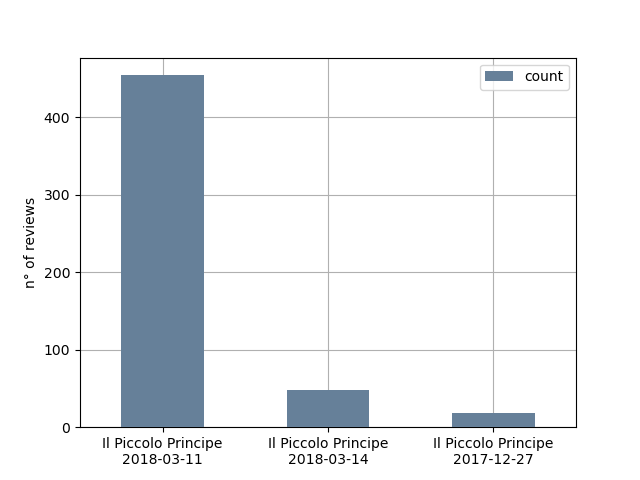
\includegraphics[width=0.6\linewidth]{img/piccolo_prin_editions.png}
	\caption{\textit{n° of review for each "Il Piccolo Principe" edition}}
\end{figure}


\noindent I accomplished this task by using ASUM, a model to perform aspect-based sentiment analysis, with the objective of discovering both the positive and negative aspects. To carry out this study I focused my attention only on the reviews of the most reviewed edition of the book "Il Piccolo Principe", so I went from the original 36035 book reviews to 454. 
The most important information of the dataset are the title and the body of the reviews. In particular, in this phase I merged these two columns into one, because the title contains a lot of useful information about the review. Moreover, I selected only the verified reviews (those written by people who actually bought the book) and they represent the 83\% of the total reviews, thus 379.

\subsection{Preprocessing}
%The workflow consists of two areas, a phase of data manipulation through Python and a phase of data processing through the ASUM model for sentiment analysis.
Before diving into the aspect based sentiment analysis, a preprocessing phase was required. First of all, the fields deemed superfluous for analysis have been removed from the dataset.

\noindent The manipualtion of the data was done sequentially and with standard steps for this kind of analyzes. For each sentence these steps of preprocessing were applied:

\begin{figure}[H]
	\centering
	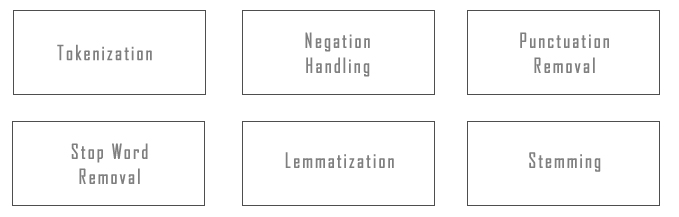
\includegraphics[width=1\linewidth]{img/preproc.jpg}
	\caption{\textit{Preprocessing phases}}
\end{figure}

\noindent The first phase was tokenization: each of the 379 reviews was tokenized into a list of phrases through the NLTK python library.

\noindent In first instance, since they can reverse the sentiment of the sentence, I decided to handle the negations simply placing the not\_ tag in front of all the words that followed the word “non” or the first adversative copulative word  up to the first punctuation mark, such as: 

\noindent ["non","ma","però","invece","anzi","bensì","tuttavia","nondimeno","pure","eppure"]

\noindent After seeing the results I thought this approach was not the best, because they were almost meaningless. Thus, I reduced the list of the negated words to only the "non", since especially for the other words it's very common in italian to have these followed by positive words; negating those i would get a completely negative review while originally the first half of the sentence was negative but the second half was positive. Nevertheless, also in this case I saw strange cases of nouns or verbs that should be complementary but were inside the same aspect (e.g "libro" and "not\_libro"). For this reason I decided to apply the negation only to adjectives, that led in better final results. \\

\noindent As regards the lemmatization phase, I tried first to apply stemming without lemmatization, but this resulted very inaccurate because Italian verbs have different tenses and, thus, many different tokens related to the same verb
were produced. To obtain good results I standardized them to their infinitive form using a POS tagging called TreeTagger, that it is also able to do grammatical analysis. 

\noindent Through this TreeTagger I also handled the negations for each adjective that follows the "non" word in a sentence up to the first punctuation mark.\\ 

\noindent Finally, each sentence was tokenized to create a list of words. All the words that belong to punctuation, strange symbols and stopwords (such as articles or conjunctions, that do not actually help you understand what someone is talking about) were deleted. \\

\noindent As I scrolled through the words, a dictionary WordList.txt (necessary to run ASUM) was built. In parallel I created an indexing, such that each word in the sentences was mapped to its corresponding word from the dictionary to generate the file BagOfSentences.txt, mandatory for ASUM as input. Below is an example of document construction:

\begin{figure}[H]
	\centering
	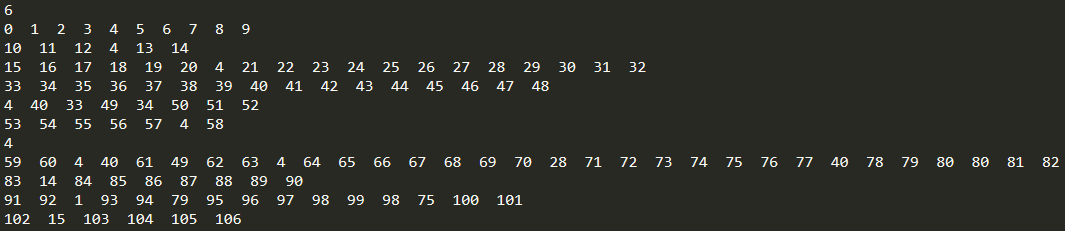
\includegraphics[width=0.9\linewidth]{img/inputBag.png}
	\caption{\textit{esempio input BagOfSentences.txt}}
\end{figure}

\noindent The first line indicates the number of phrases in the review, then there are a number of lines in which each index refers to the position of the word in the wordList. \\

\noindent According to the authors of ASUM, the model works better if the sentences within a review are composed of many words, because short sentences lack of evidence for both sentiments and aspects, and I also removed sentences that were too long.
Thus, for the analysis I removed the sentences with:
\begin{itemize}
	\item \textit{long sentences}: more than 300 words;
	\item \textit{short sentences}: less than 5 words.
\end{itemize}

\subsection{Most common words}
Before starting the experimentation with ASUM, I computed the most common words with respect to positive and negative reviews with the purpose of discovering the most used one. I divided the reviews in positive and negative, considering the number of stars: a review is positive if its number of stars is greater than 3, negative otherwise. Fig. 4 shows the most common words used in the negative reviews, while Fig. 5 shows the most common words used in the positive ones. As we can see, negative reviewers comment more the shipment and the quality of the cover, while the positive ones are more in general about the book contents and the price.

\begin{figure}[H]
	\centering
	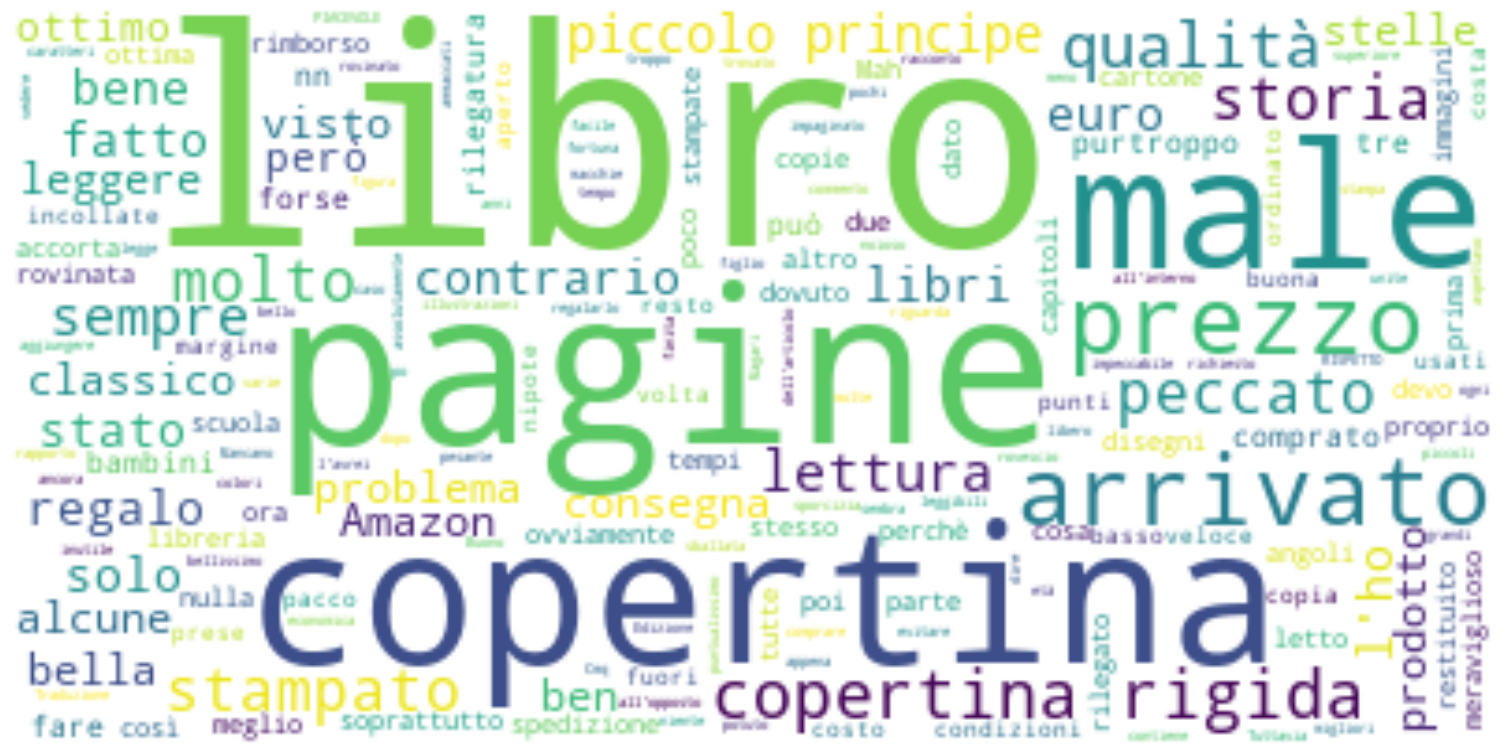
\includegraphics[width=0.9\linewidth]{img/bad_words.jpg}
	\caption{\textit{The most common words used in the negative reviews}}
\end{figure}

\begin{figure}[H]
	\centering
	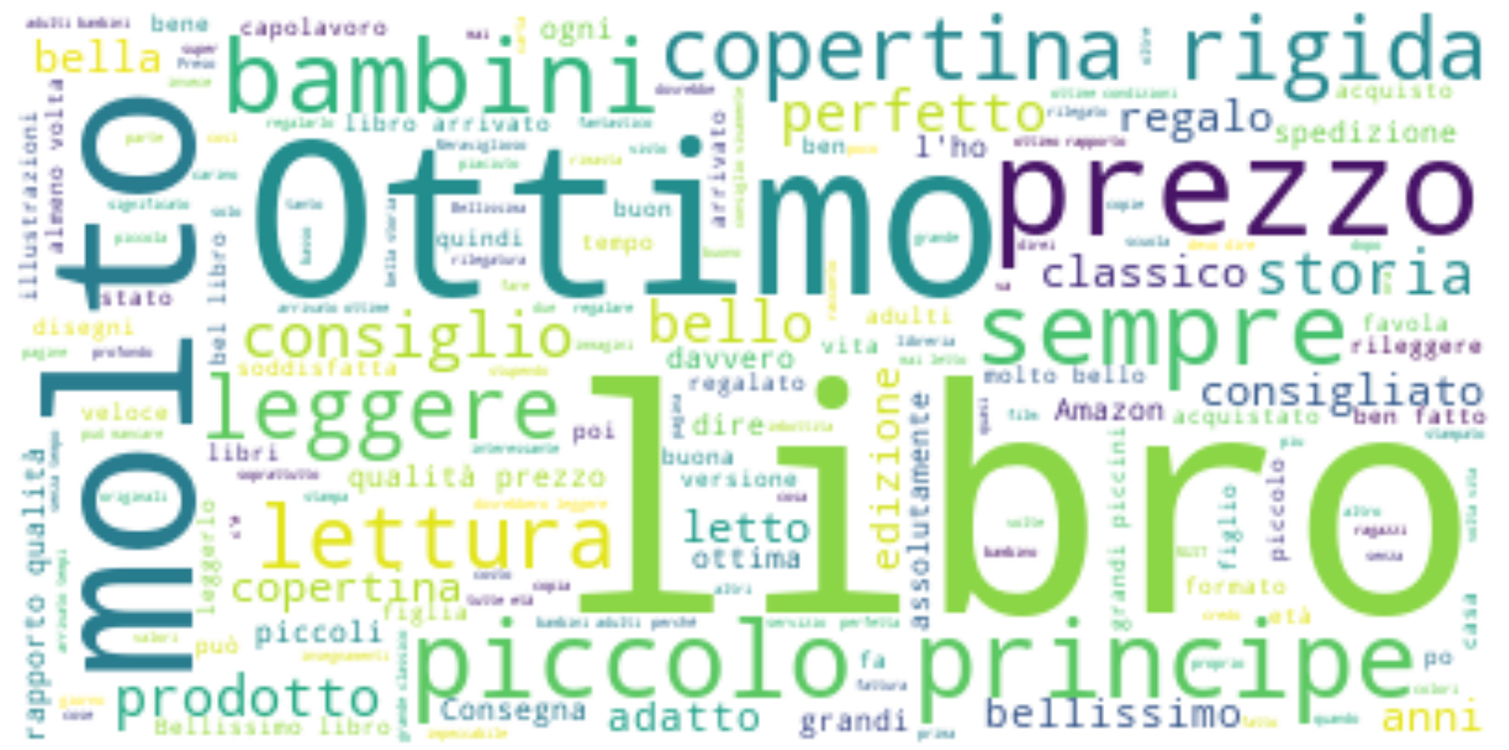
\includegraphics[width=0.9\linewidth]{img/good_words.jpg}
	\caption{\textit{The most common words used in the positive reviews}}
\end{figure}

\subsection{Sentiword seeds}
In order to help ASUM better distinguish positive words from negative ones at first I provided it with two lists of words found on github at this \href{https://github.com/gragusa/sentiment-lang-italian}{\textbf{link}}. There are 3052 negative words and 1382 positive words. Despite the large number of good positive aspects as output, I cannot say that I have achieved good results because the aspects of negative sentiment were not very clear. 
%For example, the word "ubriacone", that refers to a character of the book, had an high probability to appear as a negative topic, but this not means it was a critique to the book.  
Thus I thought to build my personal list, with these positive words:\\
\begin{center}
	\begin{tabular}{ |c c c c c| } 
		\hline
		soddisfatto & appassionante & raccomandare & favola & simpatico\\ 
		bambino & dolce & wow & consiglio & consigliato\\ 
		soddisfatto & meraviglioso & magnifico & perfetto & ottimo\\ 
		buono & buon & super & top & godibile\\ 
		regalo & raccomandato & speciale & ricordo & acquisto\\ 
		classico & figlio & adulto & molto & storia\\ 
		rileggere & veloce & amo & acquistare & copertina\\ 
		prodotto & copia & not\_brutto & not\_brutta & not\_triste\\ 
		not\_tristemente & not\_tristezza & not\_inadatto & bello & emozionante\\ 
		\hline
	\end{tabular}
\end{center}
\newpage
\noindent And these negative words:
\begin{center}
	\begin{tabular}{ |c c c c c| } 
		\hline
		costoso & brutto & ritardo & rovinato & rotto\\ 
		orribile & orrendo & noioso & schifo & ripetitivo\\ 
		vomitare & problema & inutile & ridicolo & senza\\ 
		danneggiato & sporcizia & sporco & deformare & deformato\\ 
		vecchio & male & strappato & evitare & danno\\ 
		difetto & difettoso & infantile & confuso & banale\\ 
		impossibile & negativo & purtroppo & confusionario & amaro\\ 
		noia & difficile & illeggibile & not\_adorare & not\_adorato\\ 
		not\_bella & not\_bellezza & not\_bellissima & not\_bellissimo & not\_bello\\ 
		not\_ben & not\_bene & not\_allegria & not\_allegro & not\_amicizia\\
		not\_apprezza & not\_apprezzabile & not\_apprezzamento & not\_apprezzare & not\_apprezzato\\
		not\_appropriato & not\_felicità & not\_fedeltà & not\_felice & not\_felicemente\\ 
		not\_felici & not\_felicissimo & not\_felicitarsi & not\_geniale & not\_consiglio\\ 
		not\_consigliato & not\_gioia & not\_lodevole & not\_splendidamente & not\_splendido\\ 
		not\_squisito & not\_successo & not\_top & not\_vero & not\_apprezzabile\\ 
		\hline
	\end{tabular}
\end{center}

\subsection{ASUM}
\noindent The ASUM output is composed by some CSVs, I focused on those related to probabilities. 
The ASUM parameters are:
\begin{itemize}
	\item \textit{t}: number of topics (aspects);
	\item \textit{s}: number of sentiments;
	\item \textit{d}: number of seed words;
	\item \textit{$\alpha$}: dirichlet prior on the document-sentiment-topic distribution;
	\item \textit{$\beta$}: dirichlet prior on the word-sentiment-topic distribution;
	\item \textit{$\gamma$}:  dirichlet prior document-sentiment distribution;
	\item \textit{i}: number of sampling iterations.
\end{itemize}

\noindent I decided to set $s=2$ because I was interested in finding only positive and negative aspects. Since about 87\% of the reviews was positive, I set $\gamma$ equal to $0.9/0.1$, where 0.9 is associated with the positive sentiment and 0.1 with the negative sentiment. Then I executed ASUM with different combinations of the remaining parameters $\alpha$, $\beta$ and $\gamma$. For each execution I manually inspected and interpreted the results. I tried with the settings $t=3, 5$ and $10$. \\

\noindent The general observed behavior is that by increasing the parameter $t$, it is possible to visualize a series of predenominant words that do not appear when using lower $t$, moreover the aspects are more defined (e.g.  with $t = 3$ words related to both shipment and edition where under the same topic). In fact, increasing $t$ we have positive aspects more connected to different emotions. The problem, however, is that as seen previously during the preprocessing phase the results of the negative aspects had almost no meaning, the reason of this may be linked to the actual number of negative topics, problems with the handling of negation or with the lexicon. \\

\noindent Increasing the number of topics up to 10 I found some duplicates within the positive aspects, actually I saw duplicates regarding the emotions of the users. With negative aspects, however, some aspects weren't truly negative, but with the right workflow they were more defined. Despite the duplicates, the results were no doubt more interesting. I did not notice any relevant differences in the results by varying of the values for $\alpha$ and $\beta$. 

\noindent In conclusion, I isolated 5 negative and 4 positive aspects. The most relevant topics, both positive and negative, are reported in the following tables:  

\begin{table}[H]
	\centering
	\begin{tabular}{|l|l|l|l|l|}
		\hline
		\multicolumn{5}{|c|}{\textbf{Positive}}                                                                                                  \\ \hline
		Edition	   & Shipment    & Classic book & Book quality & Memories                               \\ \hline
		libro      & arrivar     & libro       & libro      & uomo                            \\
		copertina  & ottimo      & bambino     & ottimo     & ricordare \\
		rigido     & buono       & lettura     & carattere  & infanzia                        \\
		ottimo     & amazon      & leggero     & leggibile  & bambino                         \\
		copia      & spedizione  & classico    & qualità    & ricordo   \\
		edizione   & veloce      & adulto      & stampa     & not\_triste                    \\
		economico  & servizio    & consigliare & lettura    & racconto  \\
		stampato   & consegna    & acquistare  & dimensione & storia    \\
		pagina     & impeccabile & rileggere   & pagina     & adulto                         \\
		rilegatura & ordinare    & regalare    & carta      & favola   \\
		\hline
	\end{tabular}
	\caption{Positive aspects}
\end{table}


\begin{table}[H]
	\centering
	\begin{tabular}{|l|l|l|l|}
		\hline
		\multicolumn{4}{|c|}{\textbf{Negative}}                               \\ \hline
		Cost              & Shipment   & Book quality & Book content \\ \hline
		libro             & ridicolo   & libro        & male         \\
		costo             & rimborso   & problema     & leggero     \\
		spendere          & amazon     & traduzione   & inutile      \\
		inutile           & problema   & pagina       & ridicolo     \\
		traduzione        & solo       & errore       & noia         \\
		qualità           & tardi      & stampa       & pensare      \\
		leggero           & spedizione & rilegare     & prezzo       \\
		noioso            & tutelare   & pessimo      & vita         \\
		not\_apprezzabile & danno      & incollare    & solo      \\
		\hline  
	\end{tabular}
	\caption{Negative aspects}
\end{table}

\noindent Finally, I have verified the results obtained by ASUM by filtering the reviews using the aspects as keywords and by manually inspecting them. 
\newpage
\section{Conclusions}
\noindent In this report I extracted valuable insights from books using a dataset containing products and reviews from the Italian Amazon market. The first goal of this project was to discover the most recommended product of the category "book" in the Amazon network and then figure out what people think about one of these, the book "Il Piccolo Principe" by Antoine de Saint-Exupéry. Concerning the first goal, I discovered that the most recommended book on Amazon is "La versione di Fenoglio". Then, I discovered that most people are very satisfied about "Il Piccolo Principe", regarding the edition, the quality of the book and it is overall considered a classic book, recommended both for adults and children, especially as a gift. There are however conflicting opinions about the shipment and the book's print quality. Some people also didn't like the book content and were not satisfied with the price.

\end{document}